\documentclass{article}
\usepackage{graphicx}
\usepackage{amsmath}
\usepackage{listings}
\usepackage{caption}
\usepackage[hidelinks]{hyperref}
\setlength{\parindent}{0pt}
\usepackage{pdfpages}


\begin{document}
    

\begin{titlepage}
    \vbox{ }
    \vbox{ }
    \begin{center}
        % Set course here
        % TIØ4120 - Operasjonsanalyse, grunnkurs
        % TDT4136 - Introduction to Artificial Intelligence
        
\includegraphics[width=0.40\textwidth]{NTNU_logo.png}\\[1cm]
    \textsc{\Large TIØ4120 - Operasjonsanalyse, grunnkurs}\\[0.5cm]
    \vbox{ }
    
    % Set title here
    { \huge \bfseries Exercise \#1}\\[0.4cm]
    
    \large
    \emph{Author:}\\
    Sondre Pedersen
    \vfill
    
    {\large\today}
\end{center}
\end{titlepage}

    \captionsetup[figure]{labelformat=empty}

        
    \section*{\textbf{Oppgave 1}}
    \vspace*{12pt}\small\textbf{a)}
    \begin{figure*}[ht]
        \centering
        \includegraphics*[width=\textwidth]{img/1a.PNG}
        \caption{Mulighetsområdet med en vilkårlig valgt målfunksjon}
    \end{figure*}
    
    \vspace*{12pt}\small\textbf{b}
    
    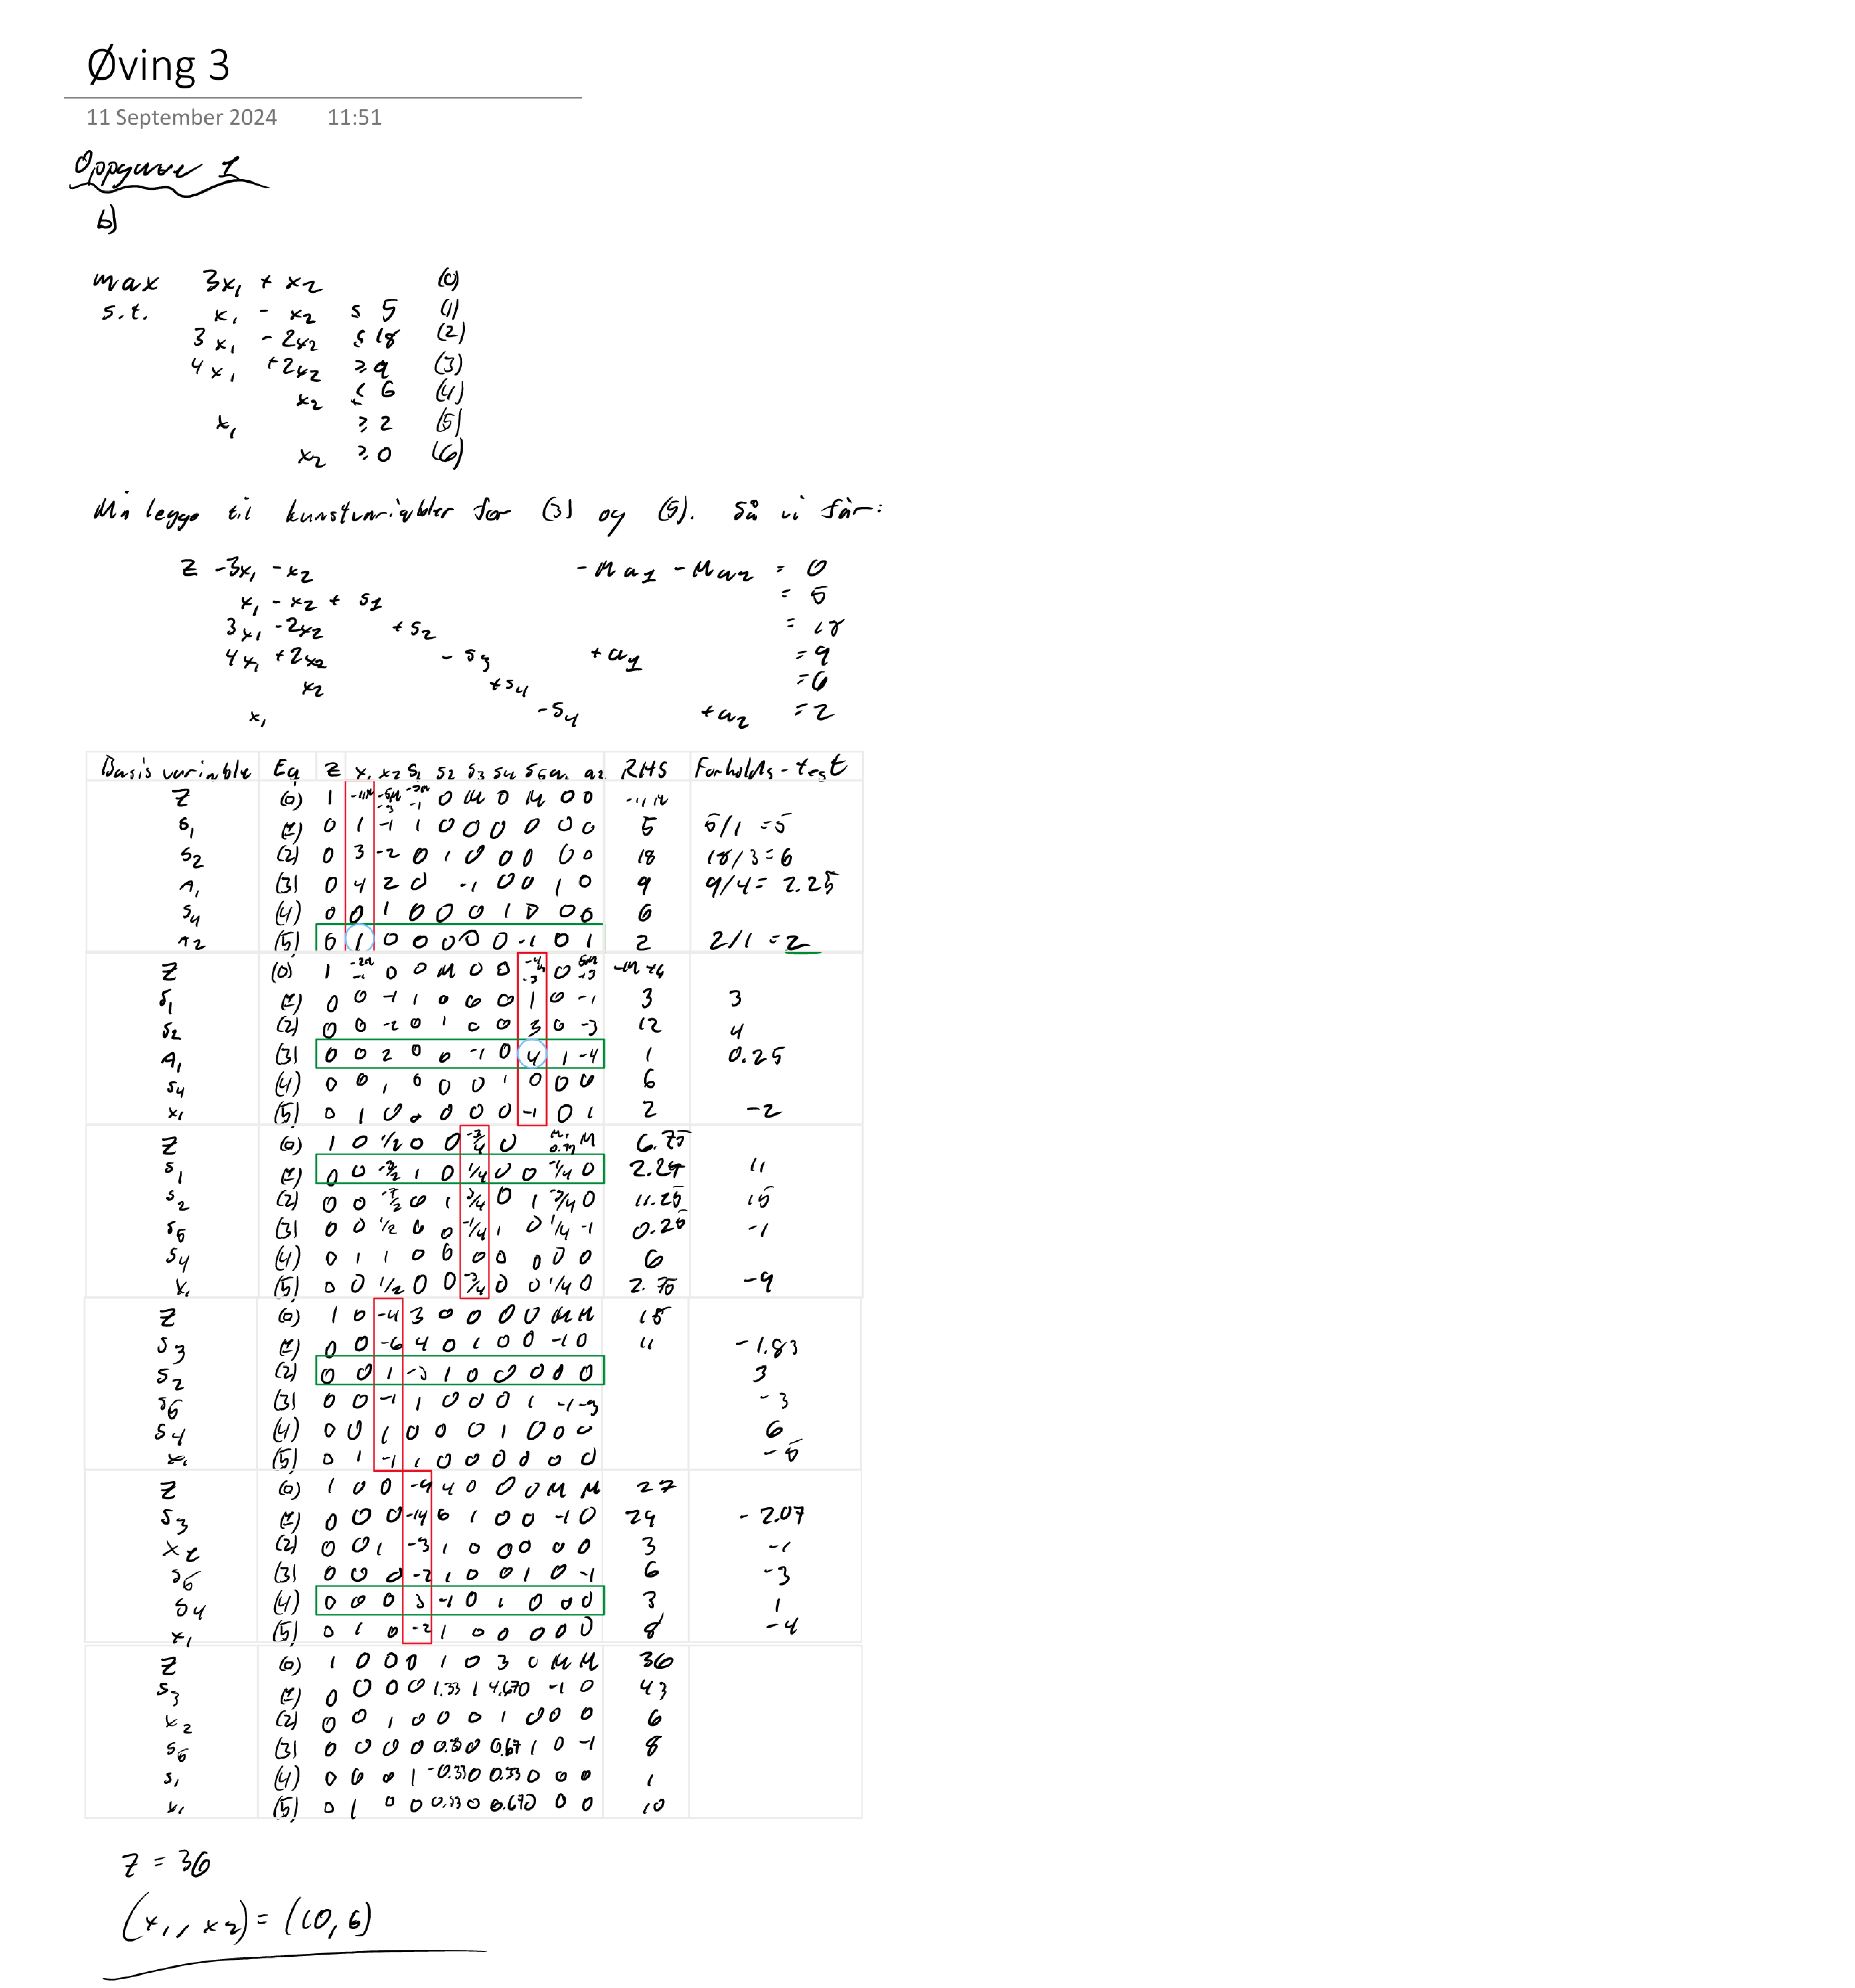
\includepdf[pages=1, trim=0 0 105mm 0, clip, width=1.6\textwidth]{oppg1.pdf}

                
    
    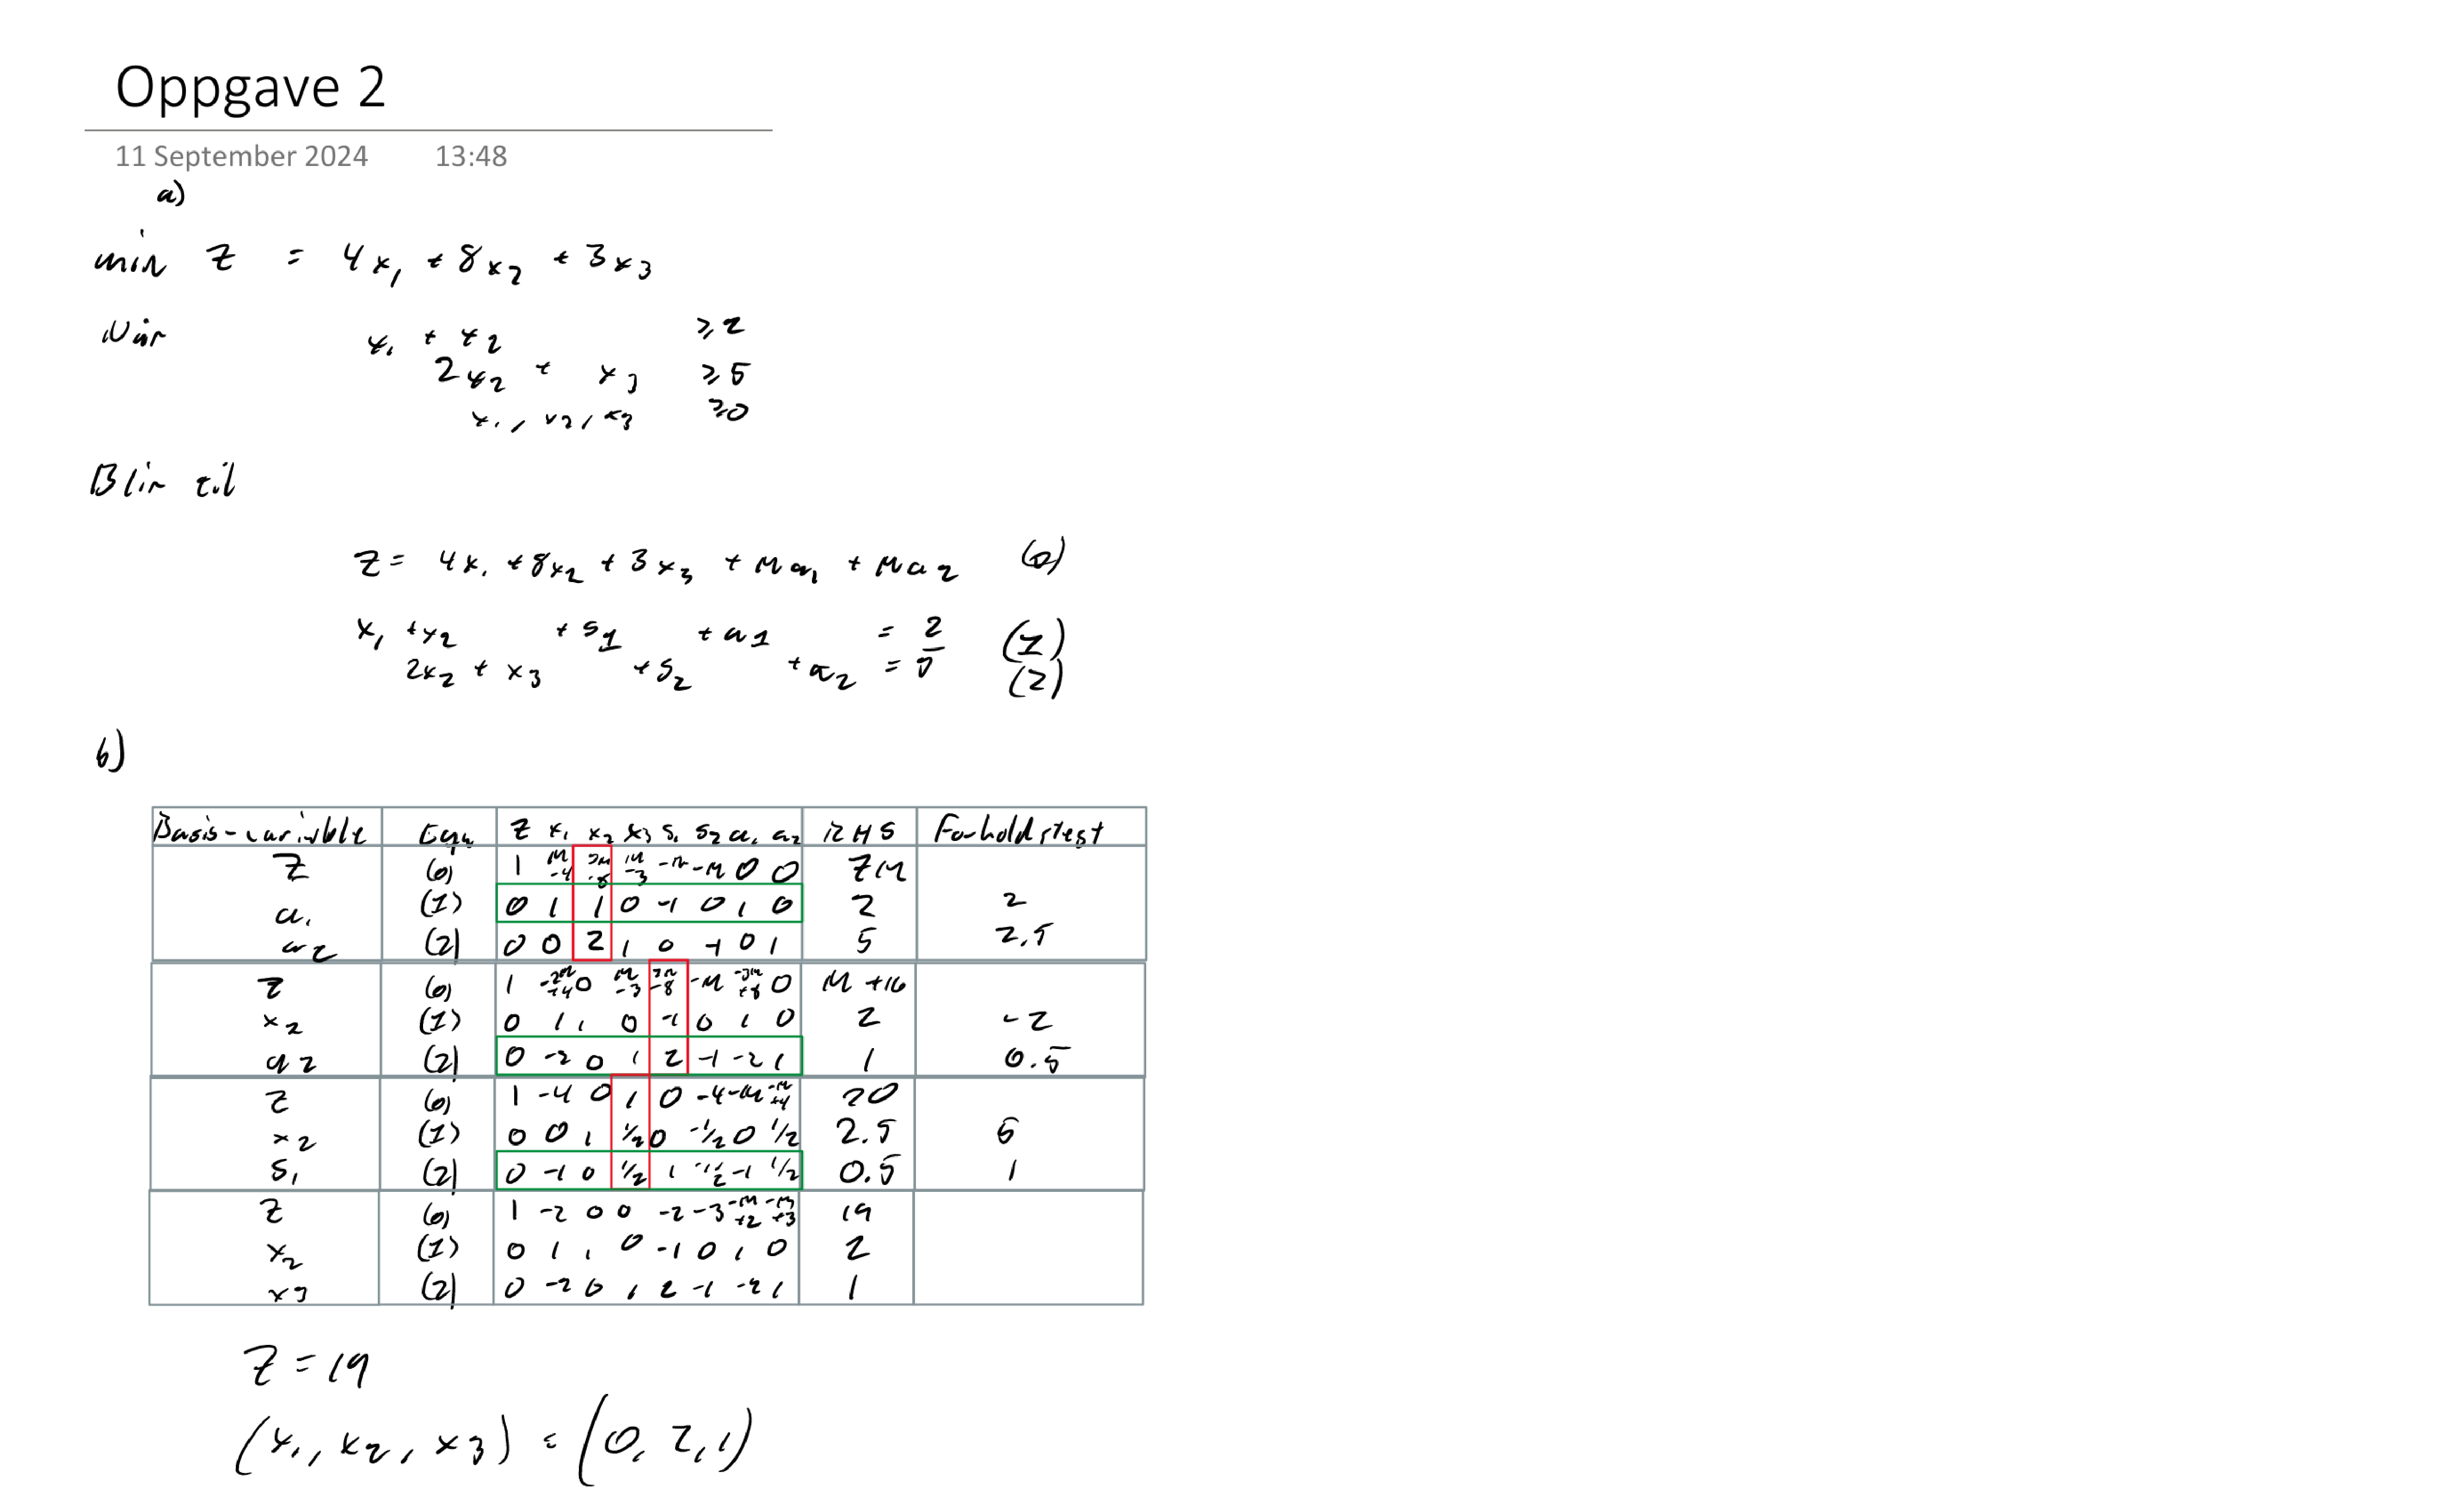
\includepdf[pages=1, trim=0 0 105mm 0, clip, width=1.6\textwidth]{Oppgave 2.pdf}

                

\end{document}